\section{Versuchsdurchführung}
\subsection{Aufbau}
Ein Querschnitt eines Geiger-Müllerzählrohrs ist in Abbildung \ref{fig:geigermuellerpic} dargestellt.
Das Geiger-Müllerzählrohr besteht aus einem metallisch einhüllenden Zylinder welcher als Kathode wirkt. 
Dieser hat den Radius $r_{k}$ und im Inneren des Zylinders befindet sich ein axial verlaufender Anodendraht mit Radius $r_{a}$.
Im Eintrittsfenster des Zählrohrs ist eine Mylarfolie angebracht, welche selbst von $\alpha$-Teilchen durchdringt werden kann. Die Zählrohre mit dieser Eigenschaft
werden auch Endfensterzählrohre genannt.
Innerhalb des Zylinders befindet sich nun ein Gasgemisch, meist bestehend aus Argon und Ethylalkohol im Verhältnis 10:1.
\begin{figure}
  \centering
  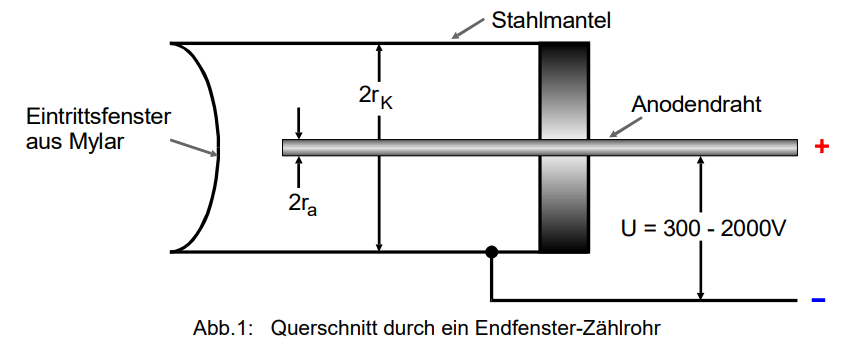
\includegraphics[width=0.7\textwidth]{bilder/Abbildung.png}
  \caption{Querschnitt eines Geiger-Müller-Zählrohres \cite{ap03}.}
  \label{fig:geigermuellerpic}
\end{figure}
\\
Anschließend wird eine Spannung von $300$-$\SI{2000}{\volt}$ zwischen die Kathode und Anode angelegt, wodurch die durch Ionisierung entstehenden Elektronen zur Anode fließen
und die nun positiv geladenen Ladungsträger zum Mantel wandern. An der Anode fließt der Elektronenstrom über einen Widerstand ab und dort erzeugt er einen Spannungsimpuls.
Anhand eines Kondensators und einem Verstärker wird dieses Signal nun letztendlich in einem Zählgerät registriert und führt auf die Anzahl der eintreffenden Teilchen im Zählrohr.
Dieses Signal lässt sich außerdem an einem Oszillographen sichtbar machen.
\newline
\\
Die Reihenfolge der Schaltelemente ist nochmal in der Abbildung \ref{fig:geigermuellerpic2} zu erkennen.
\begin{figure}
  \centering
  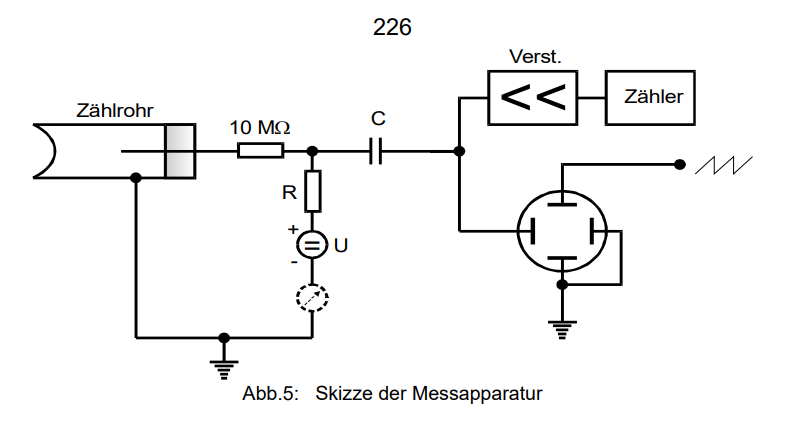
\includegraphics[width=0.7\textwidth]{bilder/Abbildung2.png}
  \caption{Skizze der Messapparatur \cite{ap03}.}
  \label{fig:geigermuellerpic2}
\end{figure}
Der Oszillograph ist dabei dem Verstärker vorgeschaltet und der Verstärker sorgt nur für einen vergrößerten Spannungsimpuls welcher am Zählgerat besser verarbeitet werden kann.
%\subsection{Funtkionsweise}
%eventuell noch Funktionsweise


\subsection{Durchführung}
Vor das Fenster des mit Mylarfolie bedeckten Zählrohrs wird eine $\beta$-Quelle platziert, hierbei wurde der $\beta$- Strahler Thalium-204 ($\ce{^{204}_{}Tl}$) verwendet. Anschließend wurde die Zählrate
am Zähler in Abhängigkeit von der angelegten Spannung abgelesen. Dabei muss stets darauf geachtet werden, dass die maximale Impulsrate nicht über $100$ $\text{Imp}/{\si{\second}}$ steigt. %siehe Theorie? maybe
\newline
\\
Gestartet wird mit der Aufnahme der Geiger-Müller Charakteristik. Dazu wird in Abständen $\increment U = \SI{10}{\volt}$ die Anzahl der Zerfälle pro Zeitintervall gemessen. Hierbei beträgt die
Messzeit pro Spannung jeweils $t = \SI{60}{\second}$.
Begonnen wurde mit einer Spannung
von $\SI{300}{\volt}$ und beendet mit $\SI{700}{\volt}$, dazu wurde jeweils eine Stromstärke $I [\si{\micro\ampere}]$ in $\SI{50}{\volt}$ Schritten an einem Amperemeter abgelesen. 
\newline
\\
Für die Bestimmung der Totzeit wird die $\ce{^{204}_{}Tl}$ Quelle näher an das Zählrohr gerückt und die Messzeit auf $\increment t = \SI{120}{\second}$ erhöht. Hierbei wird die Zwei-Quellen-Methode %siehe Theo
verwendet. Zunächst wird eine $\ce{^{204}_{}Tl}$ Quelle vor das Zählrohr platziert und die Zählrate $N_{1} [\text{Imp}/120{\si{\second}}]$ gemessen, nach $\increment t = \SI{120}{\second}$ wird dann eine Zweite Quelle 
dazugestellt und es ergibt sich die Zählrate $N_{1+2} [\text{Imp}/120{\si{\second}}]$. Abschließend wird die zweite Quelle stehen gelassen und die erste weggestellt. Nach weiteren 120 Sekunden wird
die Zählrate  $N_{2} [\text{Imp}/120{\si{\second}}]$ notiert.
\newline
\\
Die Spannungsimpulse wurden anschließend noch am Oszilloskop graphisch dargestellt und in Abbildung \ref{fig:abb4} festgehalten.